%% EAAI / Elsevier manuscript, full version with author names.
%% Source of truth for the text: OrbitGuard_paper.docx at the repository root.
%% Document class: official Elsevier elsarticle (single-column preprint).
%% Citation style: EAAI Harvard / author-year (elsarticle-harv).
%% Text changes made after the first conversion are listed in CONTENT_PRESERVATION_REPORT.md.

\documentclass[preprint,12pt,authoryear]{elsarticle}

\usepackage{amssymb}
\usepackage{amsmath}
\usepackage{booktabs}
\usepackage{graphicx}
\usepackage{tabularx}
\usepackage{url}
\usepackage{hyperref}

\journal{Engineering Applications of Artificial Intelligence}

\begin{document}

\begin{frontmatter}

\title{A Scale-Invariant Baseline Can Miss a Broken Deep Model: Grouped-Normalisation Collapse in Learned Trajectory Screening}

\author[inst1]{Harsha Vardan M Sakamuri}
\author[inst1]{Rohit Michael Raj}
\author[inst1]{Valarmathi P.\corref{cor1}}
\ead{valarmathi.sudhakar@vit.ac.in}
\cortext[cor1]{Corresponding author}
\affiliation[inst1]{organization={School of Computer Science and Engineering (SCOPE), Vellore Institute of Technology},
            addressline={Vandalur--Kelambakkam Road, Melakottaiyur},
            city={Chennai},
            postcode={600127},
            state={Tamil Nadu},
            country={India}}

\begin{abstract}
A single feature scaler is often used among a set of data. We show that it can quietly harm a sequence model while two otherwise sensible checks, a mixed-group validation score and the particular scale-invariant XGBoost baseline tested here, remain healthy. A Transformer trained with a scaler averaged over a target group ceases to react to the input on Venus (3.11e-05 prediction standard deviation on unseen missions, 0.6037 validation area under the ROC curve (AUC)). The same transformed arrays remain almost perfectly separable by XGBoost, whose AUC varies by at most 0.0002 across the three normalisation settings. This is a narrow invariance result, not a claim that tree models generally cannot diagnose preprocessing errors. The failure is selective: 1 of 4 targets collapses; the remaining targets lose between 0.0003 and 0.0925 AUC while continuing to discriminate. Collapse occurs on 4 of 5 seeds, so five seeds do not establish universal reliability. Our AI contribution is a controlled test of when pooled normalisation breaks a sequence model, and a prediction-spread statistic that needs no labels at inference and exposes the failure, with its threshold set on validation runs. On NASA turbofan data the signal also shrinks about nine times, but the model keeps working. The engineering application is screening simulated spacecraft trajectories to save compute; operational integration is proposed, not flight-demonstrated.
\end{abstract}

%% Graphical abstract: optional, not supplied. If one is made, upload it as a
%% separate file (531 x 1328 pixels, height by width, or proportionally more).
%% Highlights: submitted as the separate file highlights.docx, as the journal asks.

\begin{keyword}
feature normalisation \sep shortcut learning \sep model diagnostics \sep simulation screening \sep trajectory analysis \sep negative results
\end{keyword}

\end{frontmatter}

\section{Introduction}
\label{sec:intro}

In Monte Carlo trajectory campaigns, the majority of the compute is used on runs that were already sure to fail when they left the parking orbit. These campaigns are a regular occurrence at flight facilities, such as the large dispersion campaign that TESS used to set its trajectory design \citep{nickel2016}. Not only is this expensive, a body of work has been developed to make each propagation even less expensive \citep{massari2017,jia2022}. Another, and obvious, approach is to steer clear of these runs: track the first part of a trajectory and cancel out the ones that will fail. It's a screen we have made. It revealed a failure that we believe is much more than astrodynamics related.

This paper deals with that failure. Grouped data was used for training the model and a single feature scaler was fitted for the entire group. It ended up emitting a single constant per group. It's not the surprising part that it happened. What's most interesting is the length of time it took to be noticed. With a mixed validation set it looked fine, since a model can score well if it differentiates groups but cannot differentiate anything within the groups, and validation AUC remained high. A baseline run was executed with a gradient boosted model, with almost perfect results, because the trees divide on the actual values and the scaling on which the network depends is not important to them. Both of the tests we would have used would have told us that the pipeline was healthy.

This isn't, of course, comfortable, as running a simple baseline is good advice. It is common practice for tabular and physical data to be checked by tree ensembles and they are often a strong choice \citep{chen2016,grinsztajn2022,shwartz2022}. In our controlled comparison, the particular XGBoost baseline is invariant to the monotone rescaling that damages the network, so its success does not test whether this network can use the compressed signal. Other tree-based checks, other feature audits, or trees exposed to a non-monotone or information-destroying preprocessing error could diagnose other failures; our evidence does not say otherwise.

Someone could say that this is only a bad scaling choice. It is, and the fix is easy. The fix is not what we are writing about. We are writing about how this failure hides. The usual validation does not show it, and the usual baseline cannot show it. We describe the failure, show why those two checks miss it, and give a check that does not miss it.

We make three contributions. It is first a controlled decomposition of the collapse, which distinguishes pooling over time from pooling across groups, and shows only the latter to be deadly. Second, a demonstration that a scale-invariant baseline actually approves of the broken configuration, as well as an inexpensive diagnostic, the spread of the predictions, that does notice it. Its threshold is set on validation runs and tested on runs it has not seen. Third, a second dataset, NASA turbofan engines, where the signal shrinks in the same way and the model keeps working, which shows that the shrinking alone is not the problem.

This paper is based on scripts in the attached repository that generate all the numbers, which are written to machine-readable artefacts. Those artefacts are then used to create the paper containing tables and figures.

\section{Related Work}
\label{sec:related}

Normalisation is crucial for training deep networks, and there are standard layers (batch, layer, group, instance) that solve a version of the problem \citep{ioffe2015,ba2016,wu2018,ulyanov2016,huang2023}. It has been long known that the ability of a network to train, and not merely the rate at which it trains, depends on the scaling of the inputs \citep{sola1997}. These layers also make some assumptions about the input that they're given. They assume that the feature statistics are stationary, or that they're comparable within each pooling axis. When more than one set of data is measured on the same scaler, but the range of the data is very different, that assumption is already broken before the first layer runs. Normalisation has also been studied for time series on its own. ST-Norm splits it into a temporal part and a spatial part for forecasting models \citep{deng2021}, and Deep Adaptive Input Normalization learns the scaling from the data \citep{passalis2020}. Those papers want a more accurate model. We ask a different question: how can a bad scaling choice break a model without anyone noticing? What we add is a controlled decomposition that shows us that it is not the pooling in general that does the damage, but only the pooling across the groups, and then an observation that the resulting model is not a weak model, but a constant model.

When a shortcut is there, a network will easily learn the easy signals and take the shortcut over the intended structure \citep{geirhos2020,shah2020}. Previous research on Clever-Hans behaviour demonstrates that the models achieve good scores for reasons that are not related to the task \citep{lapuschkin2019}. If the scales are grouped and are not homogenous, there is an exceptionally clean shortcut, the distance between the group centroids. This type of model simply memorizes the difference, and has validation AUC of $>$0.95 but performs no better inside individual groups. That's what we saw. Here, our contribution is a diagnostic (spread of the predictions within a group) which does not need any label and is quite different from the common underfitting. It is also not a modelling problem, but a pipeline level problem, like many which can be found in the shared preprocessing code that no single model owns \citep{chaudhary2018}.

Tree ensembles perform well on tabular and physical data, and often perform with the same or better results than deep models \citep{chen2016,grinsztajn2022,shwartz2022,ke2017,pasaribu2024}, and many practitioners turn to a tree as a baseline for that reason. Their splits are axis-aligned and threshold-based, so a monotone rescaling can preserve the available ordering. That useful invariance is why the tested XGBoost baseline misses this particular cross-group scaling failure when it receives the same transformed arrays; it does not imply that tree baselines are generally unable to identify preprocessing errors.

The word `collapse' also needs disambiguation. Neural collapse conventionally describes the terminal-phase geometry of within-class representations and classifiers after training error vanishes \citep{papyan2020}; our outcome is different: predictions over distinct missions become nearly constant after cross-group scaling. Work on predictive uncertainty under shift shows that confidence and calibration can deteriorate when the deployment distribution changes \citep{ovadia2019}, while two-sample tests can detect changes between reference and incoming feature distributions without target labels \citep{rabanser2019}. Production-readiness rubrics likewise call for data, model, and serving-pipeline monitors rather than relying on a single held-out score \citep{breck2017}. Table~\ref{tab:related-comparison} makes these boundaries explicit.

\begin{table*}[t]
\centering
\caption{Comparison with adjacent diagnostics. Label-free inference does not remove the need for development-time threshold calibration and evaluation.}
\label{tab:related-comparison}
\scriptsize
\renewcommand{\arraystretch}{0.9}
\setlength{\tabcolsep}{3pt}
\begin{tabularx}{\textwidth}{@{}p{0.17\textwidth}p{0.20\textwidth}p{0.16\textwidth}p{0.15\textwidth}X@{}}
\toprule
Prior method & Failure detected & Label requirement & Dependence on a reference model & Limitation addressed by our approach \\
\midrule
Neural-collapse geometry \citep{papyan2020} & Terminal class-feature geometry & Class labels; internal activations & No external model & Targets output constancy from grouped preprocessing, not terminal-phase geometry. \\
Predictive uncertainty \citep{ovadia2019} & Uncertainty and calibration under shift & Labels for evaluation & Method-dependent; often ensembles & Directly tests a distinct output degeneracy. \\
Dataset-shift tests \citep{rabanser2019} & Source--target distribution change & No target labels for alarm & Reference distribution; sometimes a domain classifier & Tests within-group model outputs, not only input shift. \\
ML pipeline validation \citep{breck2017} & Broad data, training, serving regressions & Test-dependent & Schema, baseline, or prior version & Supplies a concrete group-level output invariant. \\
This work & Near-constant within-group predictions & None to compute; labels to calibrate/evaluate & None for spread; optional XGBoost triage & Isolates cross-target pooling and separates collapse from low AUC. \\
\bottomrule
\end{tabularx}
\end{table*}

Networks have been successfully applied in astrodynamics for trajectory optimization, approximation of optimal control \citep{izzo2019survey,izzo2024,sanchez2018}, cost estimation without complete propagation \citep{li2020deep,izzo2019ml} and learning of a robust low thrust policy with certification via Monte Carlo \citep{zavoli2021}. Learned models also correct orbit predictions from sparse tracking \citep{li2020orbit}, stand in for Monte Carlo when propagating orbit uncertainty forward \citep{zhou2024}, and are used for anomaly and fault detection in spacecraft telemetry \citep{ibrahim2019,naik2020}, where the same family of attention architectures is used as here \citep{jiang2023}. Screening specifically, by means of a learned model selecting which of a very large number of candidate cases get full analysis, is already recognized: an ESA competition on real conjunction data \citep{uriot2020,acciarini2021}, and a benchmark of deep approaches against the classical filters they would replace \citep{stevenson2023}. The final one is the most similar setting, a screening task on a deterministic astrodynamics simulator, measured against non-deep baselines. We could not find an article in this literature that considers early termination of individual Monte Carlo trajectory runs as we do in Section~\ref{sec:screen}. The closest work decreases the cost of each propagation rather than deciding which propagations to start \citep{massari2017,jia2022}. The general idea is to use a learned surrogate instead of part of an expensive simulation \citep{yin2022}.

\section{Setup}
\label{sec:setup}

In total, we developed 70,000 missions that leave the Earth, 10,000 missions to each of seven interplanetary targets (Mercury, Venus, Mars, Jupiter, Saturn, Uranus and Neptune), using NASA's General Mission Analysis Tool. It has an extensively verified two and three body propagator \citep{hughes2014}, and is deterministic. Each mission has six injection offsets, which are the components of the trans orbit insertion burn (\texttt{dv\_V}, \texttt{dv\_N}, \texttt{dv\_B}), and the RAAN, AOP and INC of the parking orbit from which the mission departs. Each is classified as success or failure, and failed ones are further sub-categorised as surface impact, orbit too high, missed target and a few others.

The interplanetary transfers are sampled at a fixed rate of 54,000 s (15 hours) and downsampled to about 100 steps for each mission. This is so that the sequences produced by targets with flight times that vary by 2 orders of magnitude are comparable. Thirteen features are recorded for each step, and include position in the synodic frame, specific orbital energy, flight path angle, normalised target distance and eccentricity. An eighth target was created (the Moon), and is intentionally left out of the study. It is a 6 day transfer inside Earth's neighbourhood, sampled at 60 s, and it doesn't have a cost structure similar to Section~\ref{sec:screen}, or a heliocentric dynamical regime.

The screening task is to observe the first 40\% of the mission's flight path and decide whether or not to abort. Splits are mission based 70/15/15, deterministic in (n, seed). The experiments are all based on a single definition in the repository, so no model is ever scored using data that was used for model selection. It is not a theoretical question. Two of the previous analyses in this project shuffled the same number of missions using the same seed, and in those analyses the same set of missions ended up in both `test' sets.

The sequence model is a Pre-LN Transformer encoder, \texttt{d\_model} 128, 8 heads, 4 layers and CLS token pooling, and 2 heads are connected to a single trunk (one for mission outcome and one for failure mode). It is trained on random length prefixes, so that its predictions are not only at the 40\% mark in the stream but at any point in the stream. The baseline is XGBoost, 300 trees at depth 5, fitted to the same normalised prefix, flattened. It is important to note that the baseline is not working from a feature set derived separately, but from the same view the network sees, which is what `the same input' means throughout this paper. That detail carries most of the argument and we're very rigid with it.

The three conditions are the following sets of normalisations, which only vary in how the feature statistics are combined. All use the same architecture, seed, split, optimiser and epoch budget.

per timestep: every one takes its statistics from the distribution of features at that timestep index, over the missions of one target (Fig.~\ref{fig:modes}). This is the configuration the working system uses.

global: one RobustScaler (median and IQR) per target, pooled across that target's own timesteps.

grouped: one RobustScaler pooled across all timesteps of all targets in a regime group (inner: Mercury, Venus, Mars; outer: Jupiter, Saturn, Uranus, Neptune). This is the setting that was not successful in production.

The third setting isn't a straw man, and here's why. You get a single RobustScaler from nearly all the standard pipeline tutorials, applied to a concatenated training set. No warning is issued and it looks like a normalised array.

\begin{figure}[t]
\centering
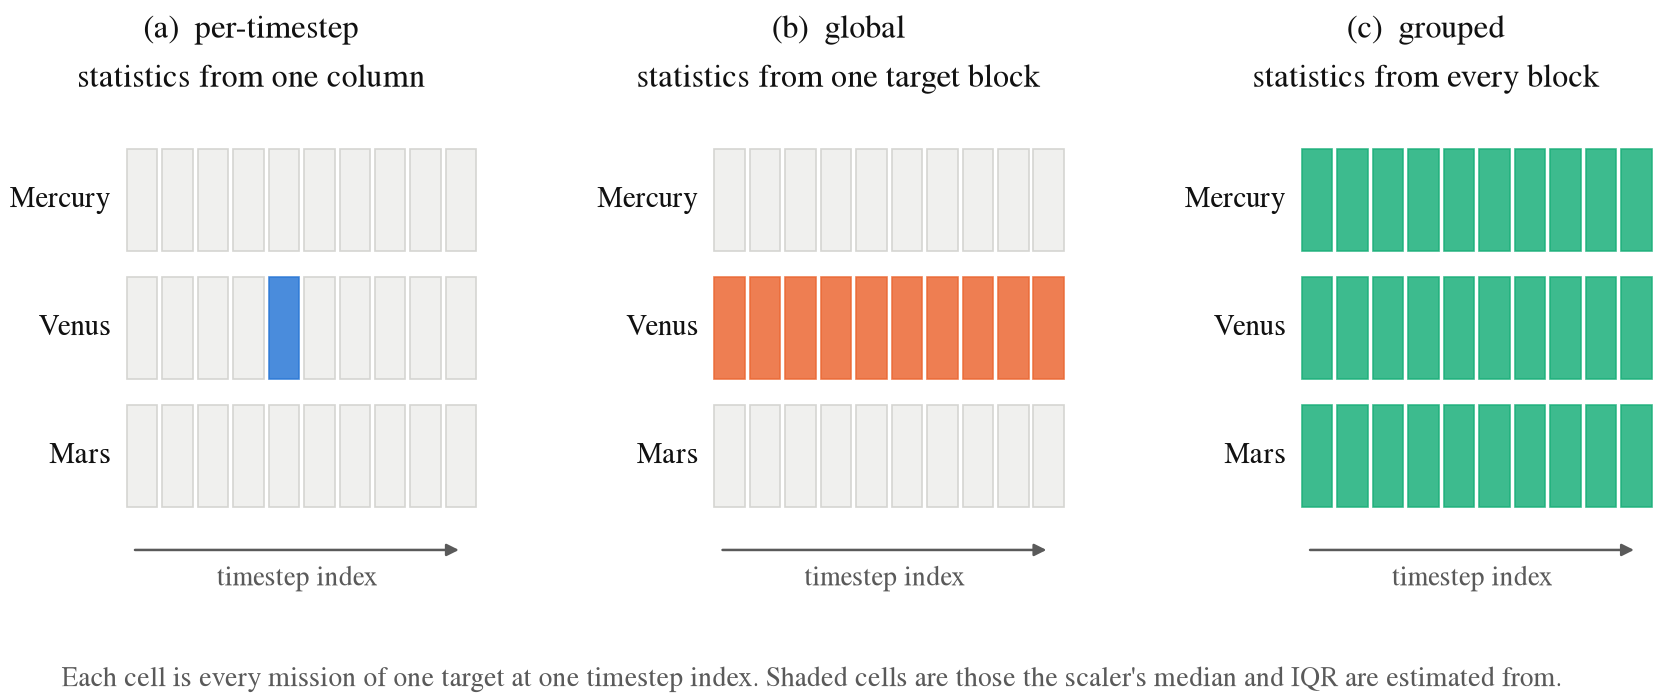
\includegraphics[width=\linewidth]{fig1.png}
\caption{The three normalisation modes, and the only difference between them: from what part of the data does the scaler get its median and IQR? Everything else in training is the same. Each cell is all the missions of one target at one timestep index, and the shaded cells are the ones the median and IQR are estimated from.}
\label{fig:modes}
\end{figure}

\section{Grouped-Normalisation Collapse}
\label{sec:collapse}

A mission's features sweep a wide range as they fly, and the range other targets occupy varies by orders of magnitude. A scaler applied to a set of pooled data will then scale the data on the scale of the largest source of variation in the set. What the screen should be able to tell apart is neither of those things. It is the spread between missions at a particular point in the flight, which by comparison is small. Pooling divides that spread by an arbitrary denominator, which drives the level of the useful signal towards zero and has no effect on the structure between groups. The network is then tasked with learning a difference that is close to the limit of what gradient descent can detect, and Pre-LN layer normalisation filters out a lot of it.

This is used as the signal ratio, defined as the average of the standard deviation of the normalised features across missions, calculated only in the observed window. It's not a limitation you would expect but it does matter. The metric is totally useless averaged over the entire flight, because late timesteps have a huge spread across missions, as the missions that fail have physically diverged by that time, and that spread swamps the early signal so that all conditions appear healthy. The model commits at 40\%, so what's important is the range within the prefix the model observes.

The first result is the decomposition that is controlled. The network is able to operate with the signal being reduced by up to a factor of 23 by pooling across time in a single target. It works on all 4 targets, with a loss of a few thousandths of AUC at most. Another kettle of fish is the pooling of a group. On Venus, the output standard deviation is 3.11e-05, which is one number for every mission, and the AUC drops from 0.9999 to 0.6037.

The term `collapse' is used instead of `underfitting' because of Fig.~\ref{fig:venus}. A low AUC on its own doesn't mean much, because that is what you would get if the model learned something poor or wrong. A distribution on unseen missions that is three ten-thousandths wide is not ambiguous at all. The network is no longer under the control of its input.

The second result is that the collapse is selective, and we report that alongside the case that breaks. In the remaining 3 targets the same manipulation leaves the output still varying, and costs between 0.0003 and 0.0925 AUC. The signal ratio is not a measure of severity either. Jupiter compresses its signal to 0.0247, whereas Mercury compresses its signal to 0.0484, and yet Jupiter loses 0.0003 AUC whilst Mercury loses 0.0925 AUC. This is because Jupiter's task is nicely split up so that even a very weak signal is sufficient. Compression is necessary for the collapse but not sufficient; how hard the underlying task is modulates it. We are not claiming that these data support a rule of the form `it collapses when the ratio is below X'. The counter example is visible in Fig.~\ref{fig:signal}.

One note on scope. This ablation isolates normalisation and no other component of the model, so only the statistics are pooled, with one model trained for each target. The production failure also shared a single trunk across the group, which compounds the problem, since one trunk then has to serve targets whose inputs have all been flattened in the same direction, towards a constant. These numbers therefore represent a minimum damage level of the configuration. They show that pooled normalisation is sufficient on its own to destroy a target, and not that this is a complete reconstruction of the original incident.

Under the grouped setting the tested XGBoost configuration reports AUC 1.0000 on Venus, the target where the network has collapsed to a constant at AUC 0.6037. Its AUC changes by at most 0.0002 across settings on all targets, which implies that this normalization choice is not visible to this baseline. It therefore establishes that discriminative ordering remains in the transformed arrays, but it does not establish that the deep model can exploit the remaining magnitude of variation.

This is the methodological part and it's crucial to pay attention to the exact claim. The information is there and this tree can use it. This particular baseline comparison is not informative on the question that has to be answered, which is `can the network use the compressed signal?'. Its invariance to this rescaling makes this check orthogonal to this defect. That statement is deliberately narrower than claiming that tree baselines cannot diagnose preprocessing errors in general.

Accuracy on a mixed validation set does not catch the collapse, because a per group constant ranks the groups correctly and a pooled metric rewards that. It's picked up by two checks.

Prediction spread within a group. For group $g$ with a batch of $n_g$ predictions, we compute $s_g=\operatorname{sd}\{P(\mathrm{fail}\mid x_i):i\in g\}$. This statistic is label-free at inference: it uses predictions and group membership, not outcomes. Labels are nevertheless needed during development to decide which low-spread states are harmful, calibrate an alert level, and estimate false alarms and missed detections.

Tested XGBoost against the network under the same preprocessing. If XGBoost has a big lead with both fed the same array, then usable ordering remains for that model while the network has failed to exploit the compressed signal.

Both are inexpensive and neither necessitates that one predicts this exact defect beforehand. In the first experiments, `collapsed' was assigned when $s_g<10^{-3}$. This rule was written into the experiment before the multi-seed replication, but after the original single run, so it is a heuristic definition and not a threshold fitted to labelled validation cases. Test labels and test AUC were not used to choose it. Labels from the same rule cannot also serve as ground truth for sensitivity or specificity, because that would be circular. Section~\ref{sec:check} therefore uses a definition based on AUC, and checks a threshold on validation and test predictions. The evidence supports the statistic as a conspicuous signature in this experiment, not $10^{-3}$ as a universal operating threshold.

\subsection{Mission-assurance interpretation and operational use}

\textbf{Demonstrated result.} Within the GMAT experiment, the group-level output statistic exposes four near-constant Venus runs that a pooled AUC and the tested XGBoost comparison do not identify. Because it checks the behaviour at the preprocessing--model interface, the same form of invariant can supplement verification and validation in other simulation-screening pipelines: it tests whether changing candidate inputs still changes the learned screen. It does not validate the trajectory propagator, prove physical correctness, certify flight software, or establish a threshold outside the evaluated configuration.

\textbf{Operational implication.} If an analogous collapse remained undetected in a mission-design campaign, the screen could assign nearly the same disposition to materially different candidates. Depending on that constant and the decision threshold, it could discard viable trajectories, retain expensive failures, distort estimates of feasible-region size, and bias trade studies or robustness margins. A healthy aggregate score from other target groups could conceal the affected group and create false confidence in the campaign. These consequences are failure analyses, not outcomes measured in a flight campaign.

\textbf{Proposed pipeline.} During development, the team would generate labelled working, degraded, and intentionally fault-injected validation states for each dataset--architecture--target-group--preprocessing version. It would calibrate a group-specific spread threshold and a minimum batch size on those validation states, freeze both before the untouched test evaluation, and record false-alarm and miss rates with uncertainty. At runtime, each screening batch would log model, scaler, data, and group versions; compute $s_g$ alongside robust spread, input-signal, and feature-shift checks; and compare only with the matching frozen limits. An alarm would quarantine the learned screen, preserve all candidates, and fall back to the full-fidelity propagation rather than aborting trajectories. An XGBoost comparison can aid offline triage by asking whether information remains in the same arrays, but is not required to compute the inference-time statistic. Once delayed outcomes are available, they would support periodic re-evaluation and versioned recalibration, and never a silent transfer of a threshold from another domain.

\begin{table}[t]
\centering
\caption{Normalisation ablation. Identical architecture, seed and split; only the pooling differs. `sig' is the mean within timestep standard deviation of the normalised features in the observed window. `std' is the standard deviation of P(fail) on unseen missions, the quantity that identifies a collapse, as against a model that is merely inaccurate.}
\label{tab:ablation}
\footnotesize
\setlength{\tabcolsep}{3.5pt}
\resizebox{\linewidth}{!}{%
\begin{tabular}{@{}l ccc ccc ccc@{}}
\toprule
 & \multicolumn{3}{c}{per-timestep} & \multicolumn{3}{c}{global} & \multicolumn{3}{c}{grouped} \\
\cmidrule(lr){2-4} \cmidrule(lr){5-7} \cmidrule(lr){8-10}
Target & sig & AUC & std & sig & AUC & std & sig & AUC & std \\
\midrule
Venus   & 0.7681 & 0.9999 & 4.72e-01 & 0.0518 & 0.9947 & 4.50e-01 & 0.0023 & 0.6037 & 3.11e-05 \\
Mars    & 1.0829 & 0.9994 & 4.33e-01 & 0.0472 & 0.9972 & 4.00e-01 & 0.8005 & 0.9422 & 4.06e-01 \\
Mercury & 0.7686 & 0.9994 & 4.27e-01 & 0.1321 & 0.9970 & 4.23e-01 & 0.0484 & 0.9069 & 4.25e-01 \\
Jupiter & 0.7708 & 1.0000 & 4.78e-01 & 0.0763 & 1.0000 & 4.78e-01 & 0.0247 & 0.9997 & 4.75e-01 \\
\bottomrule
\end{tabular}}
\end{table}

\begin{figure}[t]
\centering
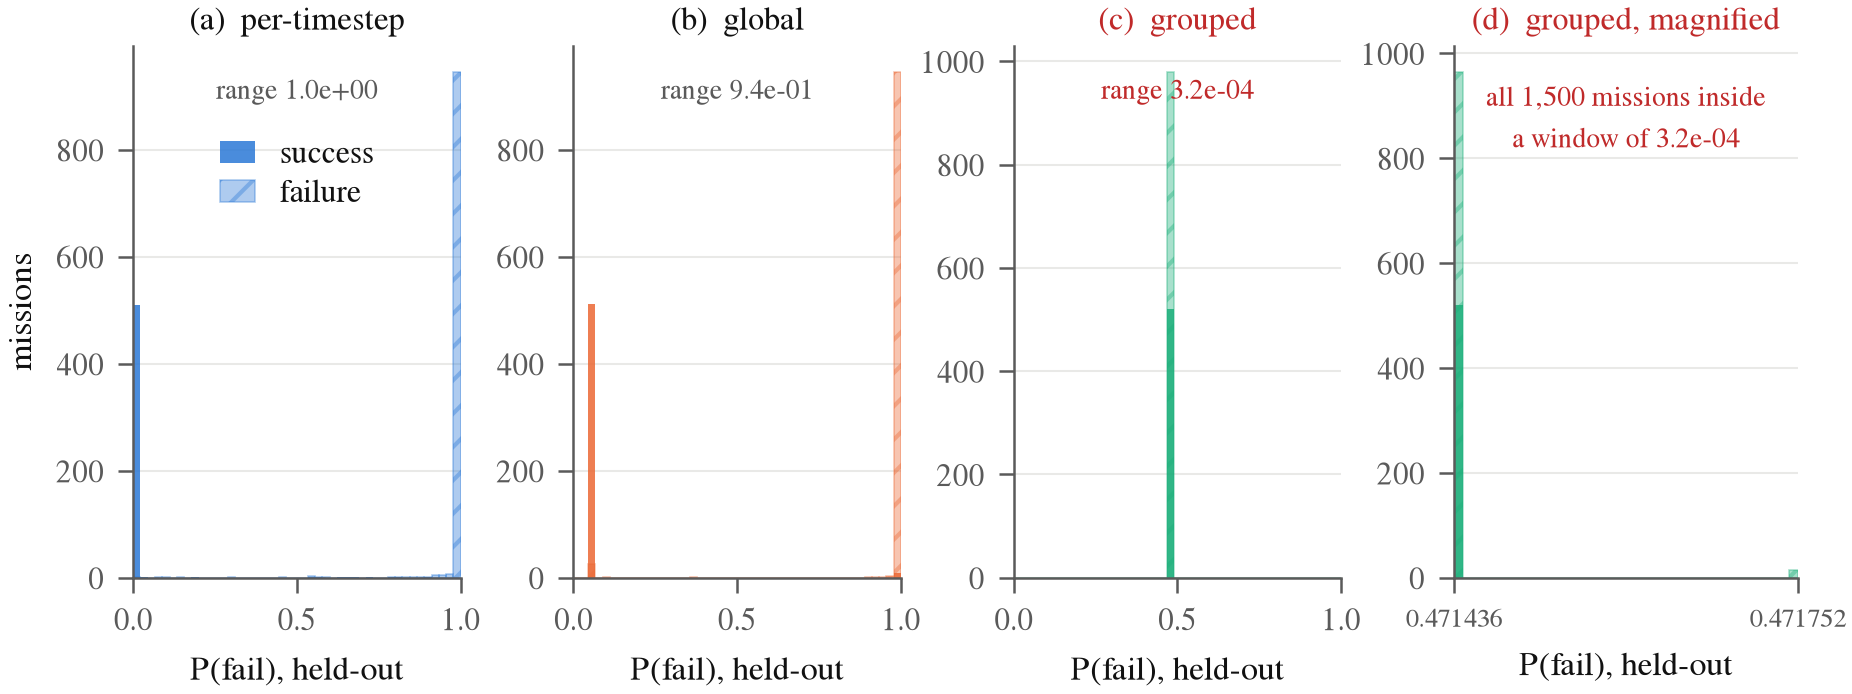
\includegraphics[width=\linewidth]{fig2.png}
\caption{P(fail) on Venus, split out for each setting. Per timestep and global normalisation put the two populations at opposite ends of the axis. Under grouped normalisation every mission gets essentially the same number. Panel (d) magnifies that spike and shows the full range covers about three ten-thousandths. This is what makes a collapse different from a merely bad model.}
\label{fig:venus}
\end{figure}

\begin{figure}[t]
\centering
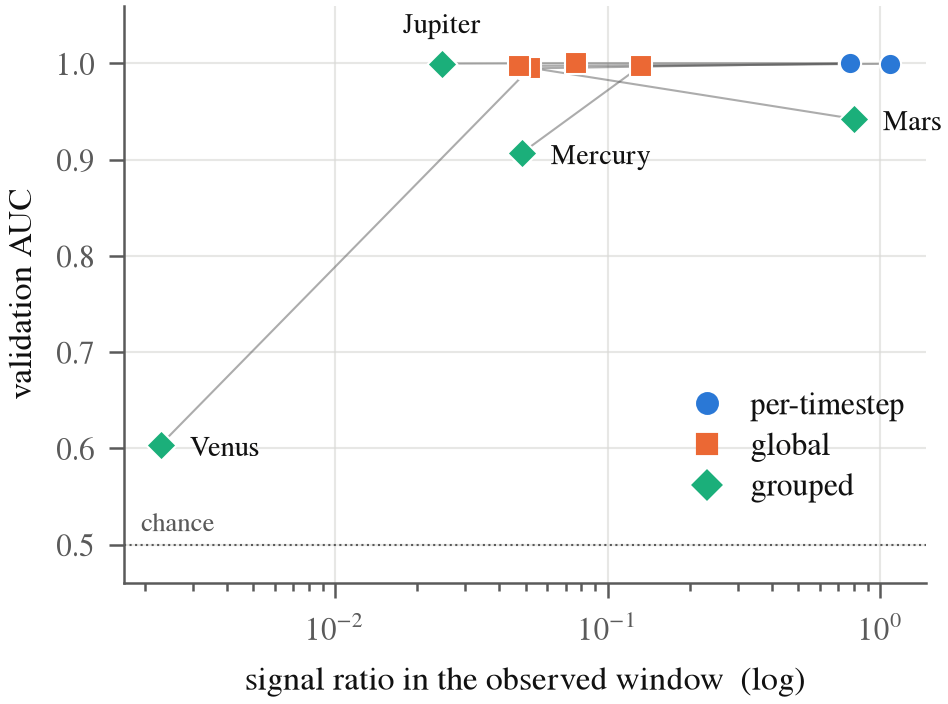
\includegraphics[width=\linewidth]{fig3.png}
\caption{Signal ratio against validation AUC. These points would lie on a curve if the collapse was only due to compression. Jupiter has a lower signal ratio than Mercury and still loses very little.}
\label{fig:signal}
\end{figure}

\begin{table}[t]
\centering
\caption{The tested XGBoost model on the same normalised window for each setting. Its AUC is nearly invariant to the particular rescaling that destroys the network.}
\label{tab:xgb}
\begin{tabular}{@{}lcccc@{}}
\toprule
Target & per-timestep & global & grouped & spread \\
\midrule
Venus   & 1.0000 & 1.0000 & 1.0000 & 0.0000 \\
Mars    & 0.9996 & 0.9998 & 0.9998 & 0.0002 \\
Mercury & 0.9997 & 0.9998 & 0.9998 & 0.0001 \\
Jupiter & 1.0000 & 1.0000 & 1.0000 & 0.0000 \\
\bottomrule
\end{tabular}
\end{table}

\begin{figure}[t]
\centering
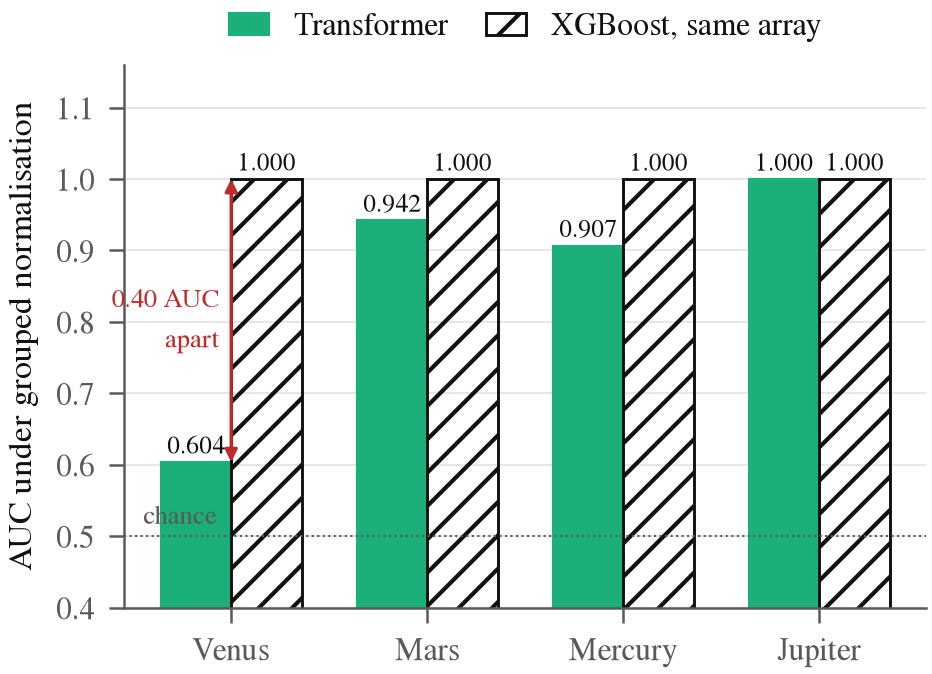
\includegraphics[width=\linewidth]{fig4.png}
\caption{Both models under grouped normalisation on the same arrays. The tested XGBoost model is at the ceiling on every target, including the one where the network is just above chance.}
\label{fig:tree}
\end{figure}

\section{Does It Reproduce Across Seeds?}
\label{sec:seeds}

Is it spread by seed? All of the above is problematic in that it's one run deep. A bad initialisation could result in an AUC of only 0.6037. Thus, we redo the whole ablation in 5 different seeds, in each of which we redraw the train/validation/test partition and the initialisation.

Compression is not dependent on seed. The signal ratio for Venus under grouped normalisation lands between 0.00222 and 0.00232 across all 5 runs, a spread of 5\% against the compression of 335x itself. The healthy condition is stable too. The difference in per timestep AUC between two different seeds is at most 0.0010. There is no seed on which Mars, Mercury or Jupiter collapse.

It depends on the seed whether the network escapes or not. Venus meets the pre-specified experimental rule $s_g<10^{-3}$ on 4 of 5 seeds, with prediction spread on unseen missions ranging from 1.57e-05 to 4.84e-05, which is 4 orders of magnitude lower than the 4.66e-01 obtained by correct normalisation. On the remaining seed it doesn't meet the collapse rule, and it doesn't recover either: prediction spread 3.64e-02, still an order of magnitude short, at AUC 0.9305 against a healthy 0.9999. The observed recurrence is 4/5, with a 95\% Wilson interval of 0.376 to 0.964. That wide interval describes recurrence of the defined state under these seeds; it is not a confidence interval for detector sensitivity and does not support universal reliability.

This is the real reason for the prediction spread diagnostic above. The range of grouped AUC for Venus over these runs is 0.5338 to 0.9305, which overlaps that of a merely weakened target. Mercury sits inside that range on every seed while still telling missions apart. AUC is thus unable to distinguish the two states. Prediction spread can. There are orders of magnitude between the collapsed runs and all the healthy runs. If you have to keep tabs on one number for this failure, watch that one.

The same invariance appears across the replication. Across 5 seeds, 4 targets and three normalisation settings, which is 60 fitted XGBoost models in total, AUC stays within 0.9989 to 1.0000, and within each seed and target the AUC difference is at most 0.0003 between settings. Thus this tested baseline does not distinguish these normalization conditions. This is evidence about one baseline--failure pairing, not all tree-based diagnostics.

\begin{table}[t]
\centering
\caption{Validation AUC across 5 seeds, mean and standard deviation, and the number of seeds on which the grouped run collapsed to a constant output.}
\label{tab:multiseed}
\begin{tabular}{@{}lccc@{}}
\toprule
Target & per-timestep AUC & grouped AUC & collapsed \\
\midrule
Venus   & $0.9998 \pm 0.0001$ & $0.6912 \pm 0.1530$ & 4/5 \\
Mars    & $0.9992 \pm 0.0004$ & $0.9457 \pm 0.0093$ & 0/5 \\
Mercury & $0.9997 \pm 0.0002$ & $0.9118 \pm 0.0036$ & 0/5 \\
Jupiter & $0.9999 \pm 0.0002$ & $0.9997 \pm 0.0003$ & 0/5 \\
\bottomrule
\end{tabular}
\end{table}

\begin{figure}[t]
\centering
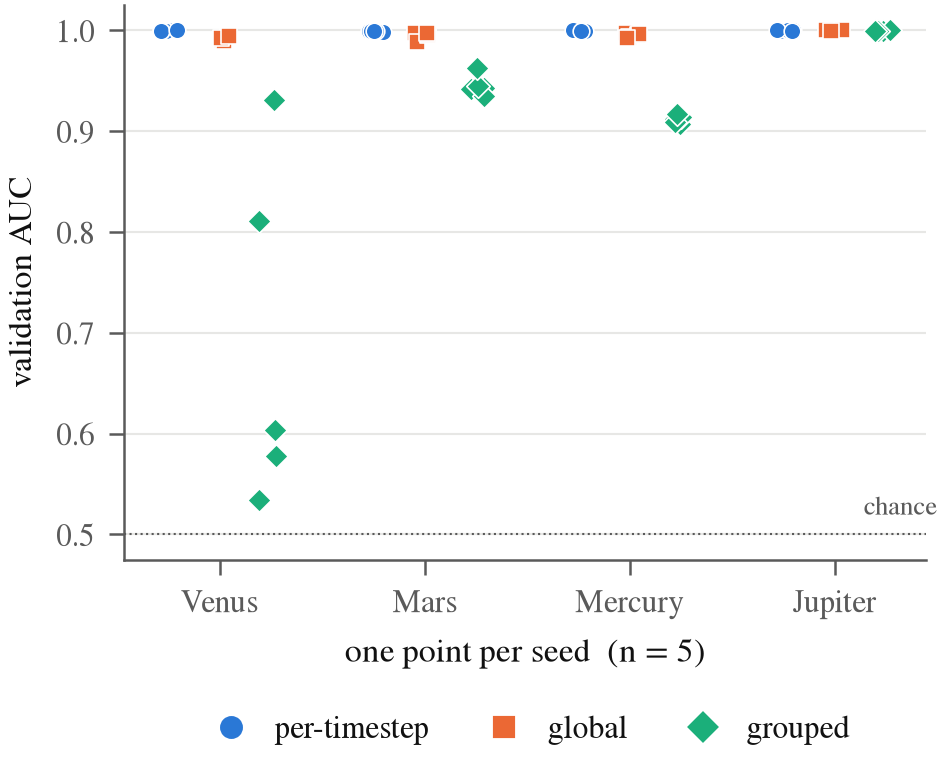
\includegraphics[width=\linewidth]{fig5.png}
\caption{Every seed plotted on its own rather than summarised as an interval. With n = 5 the spread of the raw points is the honest summary.}
\label{fig:seeds}
\end{figure}

\section{A Check That Finds the Collapse}
\label{sec:check}

A collapsed model gives nearly the same P(fail) to every mission. So we look at how much its predictions vary. The score is twice the group spread $s_g$ of Section~\ref{sec:collapse}, so that it runs from 0 to 1:
\begin{equation}
S = 2\,\mathrm{Std}(\hat{p}),
\end{equation}
where $\hat{p}$ is the predicted P(fail) on the held out missions of one target. It is 0 for a constant output, and 1 for the widest spread a probability can have. It needs no labels at inference time and no second model. Labels are used only in development, to say which runs have collapsed and to set the threshold. The four runs that this definition marks as collapsed are the same four that fall below the earlier rule $s_g<10^{-3}$.

The second score is the one a reviewer would try first. It divides by the spread of a healthy model on the same data:
\begin{equation}
D = \frac{\mathrm{Std}(\hat{p})}{\mathrm{Std}(\hat{p}_{\mathrm{healthy}}) + \epsilon}.
\end{equation}
It needs a model that was trained the right way, and when something is broken that is the thing we do not have. So we use $S$ as the main score and report $D$ to compare.

To get models in every state we repeat the ablation of Section~\ref{sec:collapse} on 5 seeds, 4 targets and 3 settings, which is 60 runs, and keep the predictions on the validation and the test missions of each run. The settings give four states. Per timestep runs are healthy. Global runs are mildly hurt. Grouped runs that keep working are severely hurt. Grouped runs that cannot rank missions are collapsed. A run counts as collapsed if its AUC on that split is 0.85 or lower. That cutoff sits in the biggest gap in the data: four runs fall between 0.51 and 0.82, and the rest are at 0.895 or above.

We chose the threshold on the validation predictions only. It is the middle, on a log scale, of the gap between the largest $S$ of a collapsed run (1.0e-04) and the smallest $S$ of a working run (0.071), which is 2.7e-03. Then we applied it, unchanged, to the test predictions. It flags 4 runs out of 60, and those are exactly the 4 that collapsed. No working run is flagged. $D$, with its threshold chosen the same way, flags the same 4. So the reference model did not add anything here.

\begin{table}[t]
\centering
\caption{The 60 runs by state. $S$ is the spread score on the test missions, and AUC is the median on the test missions. The spread of the collapsed runs is at least 750 times smaller than that of any other run.}
\label{tab:states}
\begin{tabular}{@{}lccc@{}}
\toprule
State & Runs & $S$ (smallest to largest) & Median AUC \\
\midrule
Healthy & 20 & 0.807 to 0.963 & 0.9996 \\
Mild & 20 & 0.748 to 0.962 & 0.9955 \\
Severe & 16 & 0.073 to 0.961 & 0.9430 \\
Collapsed & 4 & 3.15e-05 to 9.69e-05 & 0.5912 \\
\bottomrule
\end{tabular}
\end{table}

\begin{figure}[t]
\centering
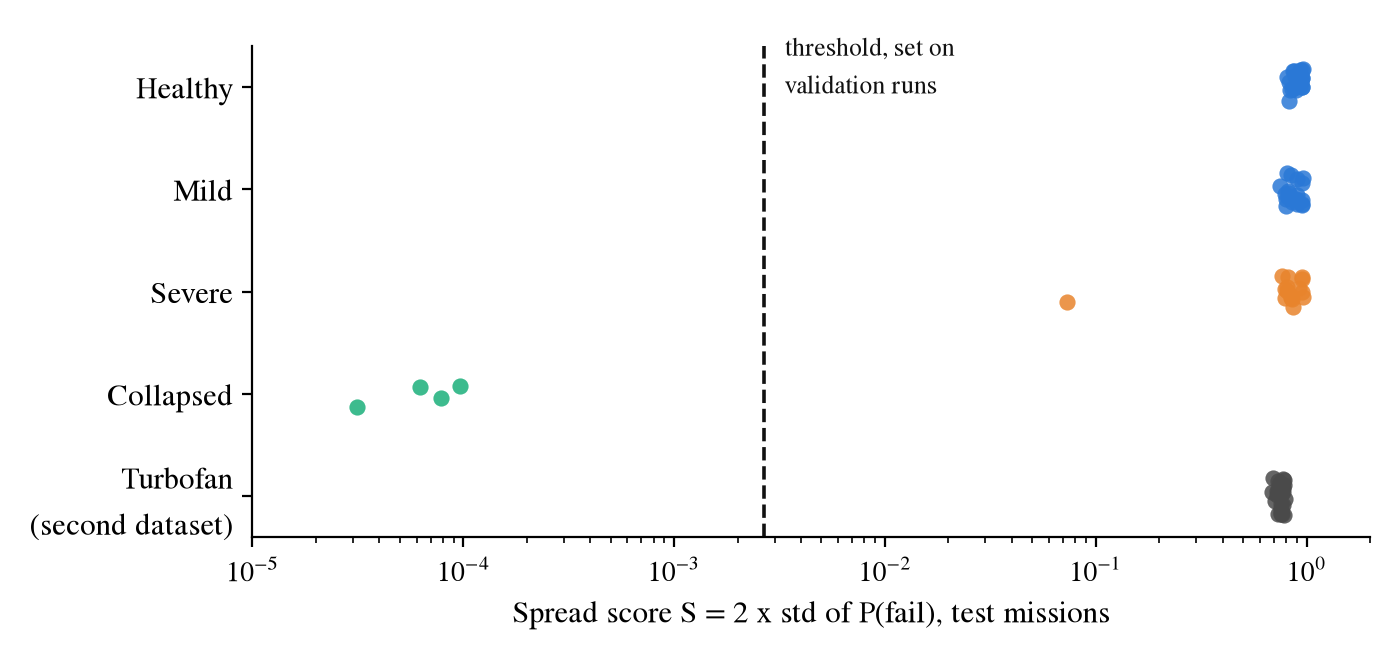
\includegraphics[width=\linewidth]{fig6.png}
\caption{The spread score of every run on the test missions. The dashed line is the threshold chosen on the validation runs. The turbofan runs of Section~\ref{sec:second} are shown for comparison, and none is flagged.}
\label{fig:check}
\end{figure}

The score is for collapse, not for every loss of accuracy. The Mercury runs under grouped normalisation lose about 0.09 AUC and their spread stays above 0.76, so the check does not flag them. Venus on seed 3 is the hard case. Its $S$ is 0.073, which is about ten times below a healthy run, and it still ranks missions at an AUC of 0.92. It is above the threshold and is not flagged. If a run is called collapsed at AUC 0.90 and not 0.85, there are 5 collapsed runs and the ROC AUC of $S$ is 0.993 and not 1.000.

The signal ratio of Section~\ref{sec:collapse} can be measured before any training. Every collapsed run has it at 0.0022 or 0.0023. Five runs are below 0.01, which are the 4 collapsed runs and Venus on seed 3, and no run at 0.0243 or above collapsed. So it works as an early warning, but it cannot say which of those runs will collapse. For that, the spread after training is needed.

\section{A Second Dataset}
\label{sec:second}

To see what happens outside our simulator we used the NASA C-MAPSS turbofan data \citep{saxena2008}, which is a standard public set for remaining useful life work \citep{li2018rul}. It has run to failure sensor records for fleets of engines. FD001 has one operating condition. FD002 and FD004 have six. The six conditions play the role the targets play in our data: the sensors sit at very different levels in each one, and the slow drift that shows an engine is wearing out is small next to that gap.

The task is to look at the last 30 cycles of an engine and say whether it will fail within 30 cycles. The split is by engine, 70/15/15, so no engine is in two sets. We scale the 14 sensors that change over an engine's life in two ways. Pooled uses one median and IQR for every row. Per group uses one for each operating condition. The model is the Transformer of Section~\ref{sec:setup}, with the same optimiser, trained for 20 epochs on 5 seeds, and the tree is XGBoost on the same scaled window. FD001 has a single condition, so the two scalings are the same thing there. It is our control.

Pooling shrinks the signal about nine times, from 0.802 to 0.083 on FD002 and from 0.859 to 0.097 on FD004. The model does not break (Table~\ref{tab:cmapss}). On both subsets the pooled Transformer is slightly ahead of the per group one, the spread of its predictions is the same, and the tree is fine either way. The check of Section~\ref{sec:check}, with the threshold it already had, flags none of the 30 runs.

\begin{table}[t]
\centering
\caption{Turbofan data, 5 seeds. `signal' is the mean within group standard deviation of the scaled features. AUC is on test engines, mean and standard deviation. $S$ is the spread score of the Transformer.}
\label{tab:cmapss}
\footnotesize
\setlength{\tabcolsep}{4pt}
\begin{tabular}{@{}llcccc@{}}
\toprule
Subset & Scaling & signal & Transformer AUC & Tree AUC & $S$ \\
\midrule
FD001 & pooled & 0.784 & $0.9916 \pm 0.0017$ & 0.9953 & 0.760 \\
FD001 & per-group & 0.784 & $0.9916 \pm 0.0017$ & 0.9953 & 0.760 \\
FD002 & pooled & 0.083 & $0.9898 \pm 0.0014$ & 0.9862 & 0.767 \\
FD002 & per-group & 0.802 & $0.9855 \pm 0.0025$ & 0.9925 & 0.755 \\
FD004 & pooled & 0.097 & $0.9910 \pm 0.0010$ & 0.9890 & 0.734 \\
FD004 & per-group & 0.859 & $0.9881 \pm 0.0044$ & 0.9933 & 0.731 \\
\bottomrule
\end{tabular}
\end{table}

This agrees with Section~\ref{sec:collapse}. The signal shrinking is not enough to break a model. In our data, Mercury and Jupiter lose most of their signal under grouped scaling and keep working. Here the drift is still there after pooling, and the model finds it. It also shows that the check does not raise an alarm on a second kind of data.

\section{Where the Screen Belongs}
\label{sec:screen}

If it has been thoroughly done on the sequence model, the real answer is that it should not be used. The six feature classifier, which is evaluated prior to any propagation whatsoever, saves 64.5\% of compute against the telemetry model's 38.3\%, at a similar cost in good missions destroyed. There is also a levelling off of accuracy between 10\% and 40\% observed. The problem is not a modelling fault. The simulator is deterministic, the outcome is a fixed function of the injection offsets, and the trajectory is an integral of the offsets. It can't transport information that the parameters don't have.

This is not to imply that the task is trivial. Logistic regression on the same 6 features achieves 0.4824 to 0.5410 AUC on all of the targets, which is chance, so the mapping between the parameters and the outcome is very nonlinear and requires a learned model. A temporal one is not really necessary. The sequential screen is only worth applying if the outcome is not known at injection: mid flight stochasticity, unmodelled dynamics, sensor noise, or campaigns where the launch parameters are not known. That is exactly the setting reinforcement learning trajectory work needs when it certifies policies through dispersed Monte Carlo campaigns \citep{zavoli2021}.

\begin{table}[t]
\centering
\caption{Screening economics. Compute is charged in propagation days, which span about a 100x range across the seven targets. Thresholds are fitted on validation and reported on the untouched test split, so the recall column is measured out of sample rather than achieved by construction.}
\label{tab:economics}
\footnotesize
\setlength{\tabcolsep}{4pt}
\begin{tabular}{@{}p{0.40\linewidth}ccc@{}}
\toprule
Screen & Compute saved & Good missions lost & Failure recall \\
\midrule
T0: six launch parameters, before propagating & 64.5\% & 0.76\% & 99.06\% \\
T40: telemetry Transformer at 40\% & 38.3\% & 0.21\% & 98.87\% \\
Cascade: T0 where confident, else T40 & 65.0\% & 1.62\% & 99.94\% \\
\bottomrule
\end{tabular}
\end{table}

For the T0 screen, an additional five-split analysis (seeds 0 to 4) gives compute saved $64.50\%\pm0.61$ percentage points, good missions lost $1.24\%\pm0.24$ percentage points, and failure recall $98.99\%\pm0.18$ percentage points (mean $\pm$ standard deviation across five splits). The T40 and cascade rows in Table~\ref{tab:economics} remain single seed-42 estimates and are not presented with an interval. The multi-seed T0 result narrows sampling uncertainty for that screen, but five correlated resplits of one synthetic corpus do not measure cross-campaign or cross-domain uncertainty.

\section{Limitations}
\label{sec:limitations}

\begin{itemize}
\item Seeds. Replication is limited to 5 seeds. The observed 4/5 recurrence has a wide 95\% Wilson interval (0.376 to 0.964), and five seeds exclude neither an unknown controlling factor nor substantial uncertainty.
\item Threshold. The cutoff that defines a collapsed run (AUC of 0.85 or lower) was chosen after the results were seen, from the largest gap in the data. The spread threshold (2.7e-03) was then set on validation predictions only and applied to the test predictions, so the test result is a check of that threshold and not a pre-registered test. All 4 collapsed runs are Venus, so only one kind of collapse has been tested. The threshold is not expected to transfer unchanged to another dataset, model architecture, output calibration, target group, prevalence or batch size. A new setting needs labelled development runs to calibrate it and an untouched test to evaluate it. The spread statistic itself needs no labels at inference time.
\item Datasets. The collapse is shown on the GMAT corpus. The turbofan data show the same signal loss without a collapse and without an alarm. That supports the absence of false alarms there, but it does not show that the threshold carries over to other domains.
\item Four targets in the ablation. 1 of 4 targets collapses, and all collapsed runs are Venus. Other target combinations and group definitions are needed to estimate how much group composition matters. The four targets agree only that the tested XGBoost AUC is nearly invariant across these normalisation settings.
\item Architecture scope. An LSTM control on the ordinary, correctly preprocessed screening task reaches test AUC 0.9928 versus 0.9958 for the Transformer, showing that the base task is not unique to one sequence architecture. The LSTM was not run under grouped normalisation, so whether this collapse generalises beyond the Transformer configuration remains open.
\item Severity range. The check flags near-constant output. It does not flag a model that loses accuracy and keeps its spread, such as Mercury. We have not built graded signal compression sweeps, so false alarms and misses over a broader range of conditions are not reported.
\item Synthetic and deterministic. There are no execution errors, no unmodelled accelerations, no sensor noise and all missions of a target have a common time base. This common time base is what makes standardisation per timestep possible at all and it is not a property of a real campaign, but of the generator.
\item Real mission data. Public satellite telemetry benchmarks exist \citep{kotowski2024,hundman2018} and are the natural next place to try the check.
\end{itemize}

\section{Conclusion}
\label{sec:conclusion}

When one scaler is pooled across groups with different scales, the tested Transformer can become a per-group constant while the tested scale-invariant XGBoost baseline still finds the same arrays separable. None of the pieces here are exotic: the defect enters through preprocessing and survives pooled validation. The exact conclusion is not that trees cannot diagnose preprocessing, but that a diagnostic invariant to this transformation cannot answer whether a magnitude-sensitive network can use the compressed signal.

We don't claim the fix, normalisation per group, to be new. The detection lesson is to monitor group-level output behaviour in addition to pooled scores and baselines. Computing prediction spread requires no inference-time labels, but turning it into a go/no-go alarm requires version-specific calibration and independent labelled evaluation during development. Our experiment demonstrates a conspicuous signature and a failure mechanism. On a second dataset, where pooling shrank the signal and the model survived, the same check raised no alarm. The mission-assurance workflow, threshold transfer study, broader severity sweep, and fall-back policy are operational implications still to be validated.

\section{Code and Data Availability}
\label{sec:code}

All the scripts for the experiments, the JSON artifacts that each number is read from, the code for the figures and the source of this document are at \url{https://github.com/Haise-727/gmat-pred}. A short map of where things are:

\begin{sloppypar}
\texttt{src/ml/} holds the experiments. \texttt{norm\_ablation.py} produces Table~\ref{tab:ablation}, \texttt{baseline\_invariance.py} Table~\ref{tab:xgb}, \texttt{diagnostic\_runs.py} with \texttt{diagnostic\_eval.py} Table~\ref{tab:states}, \texttt{second\_dataset.py} Table~\ref{tab:cmapss}, \texttt{prune\_economics.py} Table~\ref{tab:economics}, and \texttt{multi\_seed\_economics.py} the T0 uncertainty summary. The turbofan data are public, from the NASA Prognostics Center of Excellence repository, and \texttt{second\_dataset.py} reads them from a folder given on the command line. All of them share the same definition of the train/validation/test partition, in \texttt{splits.py}.
\end{sloppypar}

\texttt{src/ml/model.py} is the Transformer, and \texttt{planet\_config.py} holds the target list, the cadences and the recorded reason the Moon is excluded.

\texttt{reports/} holds the measured artifacts. Every reported number comes from one of those JSON files; \texttt{multiseed\_paper/} holds the runs behind Table~\ref{tab:multiseed}, and \texttt{prune\_economics\_multiseed.json} holds the additional T0 split-seed analysis.

\texttt{docs/RESEARCH\_LEDGER.md} is the complete decision history, including two analyses that were invalidated by a positional join and the corrections that replaced them. \texttt{docs/LIMITATIONS.md} states what the results do not support.

The JSON creates the tables and figures in this manuscript and not the other way round. No number was typed into the manuscript by hand.

The experiments read per target \texttt{.npz} files of roughly 70 MB each, which are derived from a 71 GB mission table that is too large to store in the repository. The scripts below regenerate the artifacts from those extracts. \texttt{ORBITGUARD\_DATA} points at the full table, and the economics analysis is the only experiment that needs it.

{\scriptsize
\begin{verbatim}
export ORBITGUARD_DATA=/path/to/dataset

# Primary results, seed 42
python -m src.ml.norm_ablation          # Table 2
python -m src.ml.baseline_invariance    # Table 3
python -m src.ml.diagnostic_runs        # Table 5, Fig. 6
python -m src.ml.diagnostic_eval
python -m src.ml.second_dataset --data /path/to/CMAPSSData   # Table 6
python -m src.ml.prune_economics        # Table 7

# Replication, one pass per seed (Table 4, Section 5)
for S in 0 1 2 3; do
  python -m src.ml.norm_ablation --seed $S \
      --out reports/multiseed_paper/normalisation_ablation_seed$S.json
  python -m src.ml.baseline_invariance --seed $S \
      --out reports/multiseed_paper/baseline_invariance_seed$S.json
done

# The document
python docs/paper/build/collect_traces.py   # Fig. 2 data
python docs/paper/build/figures.py          # Figs. 1 to 5
python eaai/new_results.py                  # Fig. 6
python docs/paper/build/render_latex.py     # this document
\end{verbatim}
}

\section*{Declaration of competing interest}
The authors declare that they have no known competing financial interests or personal relationships that could have appeared to influence the work reported in this paper.

\section*{CRediT authorship contribution statement}
\textbf{Harsha Vardan M Sakamuri:} Conceptualization, Methodology, Software, Validation, Formal analysis, Investigation, Data curation, Writing -- original draft, Writing -- review \& editing, Visualization, Project administration, Resources.
\textbf{Rohit Michael Raj:} Conceptualization, Methodology, Software, Validation, Formal analysis, Investigation, Data curation, Writing -- original draft, Writing -- review \& editing, Visualization, Project administration, Resources.
\textbf{Valarmathi P.:} Supervision.

\section*{Funding}
This research did not receive any specific grant from funding agencies in the public, commercial, or not-for-profit sectors.

\section*{Declaration of Generative AI and AI-assisted technologies in the writing process}
During the preparation of this work the authors used Claude (Anthropic) in order to write and debug code, draft parts of the text, and check references. After using this tool, the authors reviewed and edited the content as needed and take full responsibility for the content of the publication.

\bibliographystyle{elsarticle-harv}
\bibliography{references}

\end{document}
